\documentclass{standalone}
\usepackage{tikz}
\usetikzlibrary{patterns, positioning}

\begin{document}
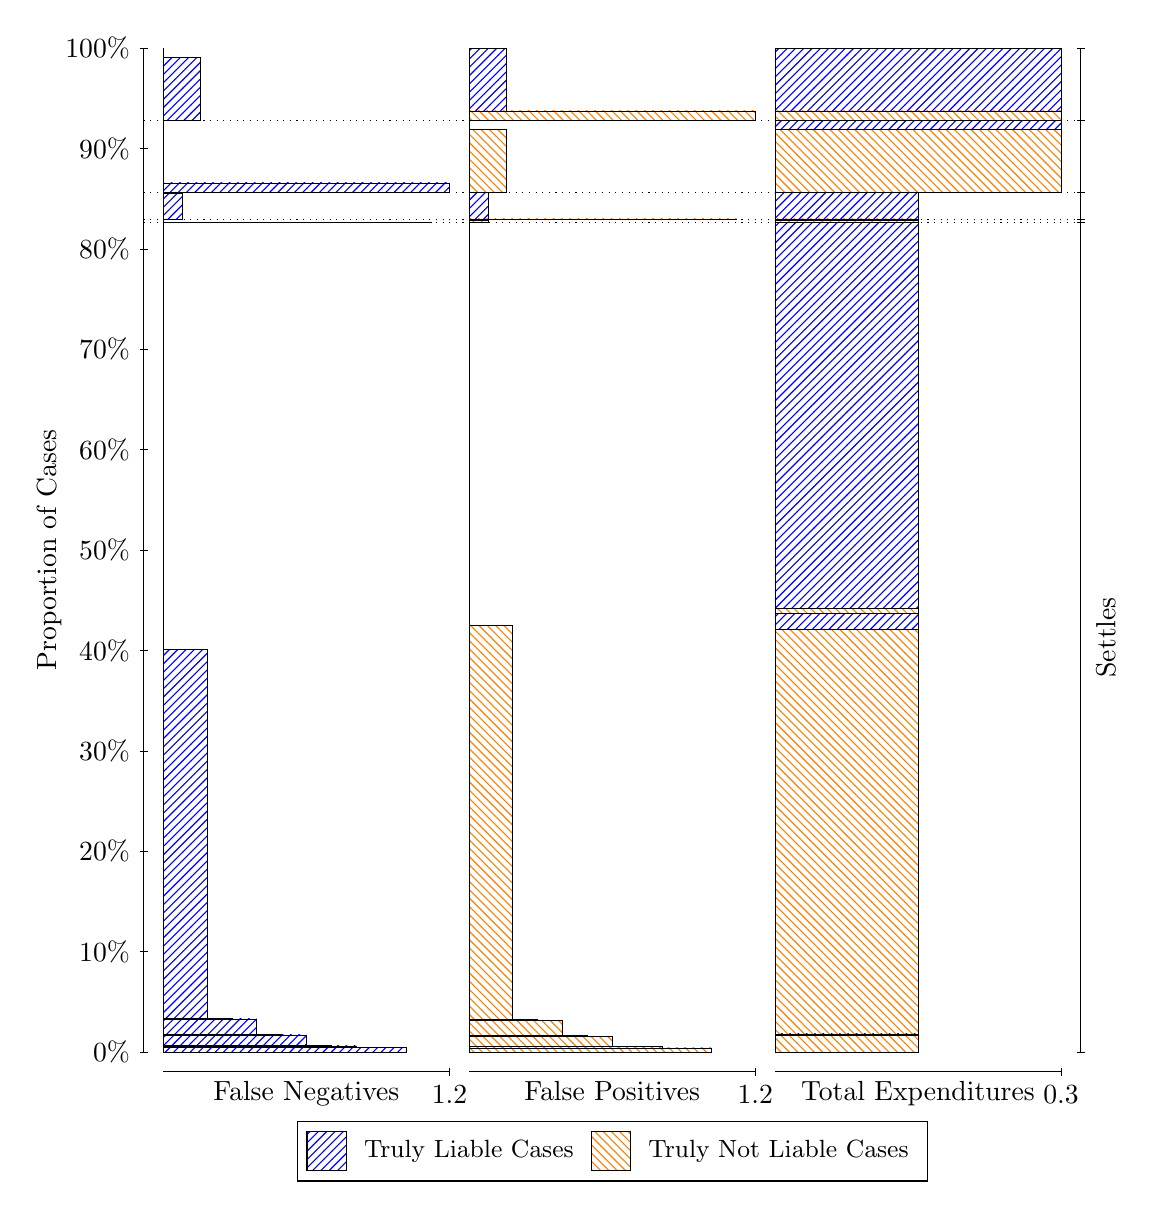
\begin{tikzpicture}
\draw[black, very thin] (1.5,1.75) -- (1.5,14.5);
\node[rotate=90, anchor=center] at (0.3, 8.125) {Proportion of Cases};
\draw[black, very thin] (1.45,1.75) -- (1.55,1.75);
\node[anchor=east] at (1.45, 1.75) {0\%};
\draw[black, very thin] (1.45,3.025) -- (1.55,3.025);
\node[anchor=east] at (1.45, 3.025) {10\%};
\draw[black, very thin] (1.45,4.3) -- (1.55,4.3);
\node[anchor=east] at (1.45, 4.3) {20\%};
\draw[black, very thin] (1.45,5.575) -- (1.55,5.575);
\node[anchor=east] at (1.45, 5.575) {30\%};
\draw[black, very thin] (1.45,6.85) -- (1.55,6.85);
\node[anchor=east] at (1.45, 6.85) {40\%};
\draw[black, very thin] (1.45,8.125) -- (1.55,8.125);
\node[anchor=east] at (1.45, 8.125) {50\%};
\draw[black, very thin] (1.45,9.4) -- (1.55,9.4);
\node[anchor=east] at (1.45, 9.4) {60\%};
\draw[black, very thin] (1.45,10.675) -- (1.55,10.675);
\node[anchor=east] at (1.45, 10.675) {70\%};
\draw[black, very thin] (1.45,11.95) -- (1.55,11.95);
\node[anchor=east] at (1.45, 11.95) {80\%};
\draw[black, very thin] (1.45,13.225) -- (1.55,13.225);
\node[anchor=east] at (1.45, 13.225) {90\%};
\draw[black, very thin] (1.45,14.5) -- (1.55,14.5);
\node[anchor=east] at (1.45, 14.5) {100\%};

\draw[black, very thin] (13.4,1.75) -- (13.4,14.5);
\draw[black, very thin] (13.35,1.75) -- (13.45,1.75);
\node[anchor=west] at (13.35, 1.75) {};
\draw[black, very thin] (13.35,12.282) -- (13.45,12.282);
\node[anchor=west] at (13.35, 12.282) {};
\draw[black, very thin] (13.35,12.32) -- (13.45,12.32);
\node[anchor=west] at (13.35, 12.32) {};
\draw[black, very thin] (13.35,12.67) -- (13.45,12.67);
\node[anchor=west] at (13.35, 12.67) {};
\draw[black, very thin] (13.35,13.585) -- (13.45,13.585);
\node[anchor=west] at (13.35, 13.585) {};
\draw[black, very thin] (13.35,14.5) -- (13.45,14.5);
\node[anchor=west] at (13.35, 14.5) {};

\draw[black, very thin, pattern color=blue, pattern=north east lines] (1.75,1.75) rectangle (4.8304,1.8081);
\draw[black, very thin, pattern color=blue, pattern=north east lines] (1.75,1.8081) rectangle (4.5145,1.8103);
\draw[black, very thin, pattern color=blue, pattern=north east lines] (1.75,1.8103) rectangle (4.1986,1.8269);
\draw[black, very thin, pattern color=blue, pattern=north east lines] (1.75,1.8269) rectangle (3.8826,1.8294);
\draw[black, very thin, pattern color=blue, pattern=north east lines] (1.75,1.8294) rectangle (3.5667,1.9666);
\draw[black, very thin, pattern color=blue, pattern=north east lines] (1.75,1.9666) rectangle (3.2507,1.974);
\draw[black, very thin, pattern color=blue, pattern=north east lines] (1.75,1.974) rectangle (2.9348,2.1698);
\draw[black, very thin, pattern color=blue, pattern=north east lines] (1.75,2.1698) rectangle (2.6188,2.1733);
\draw[black, very thin, pattern color=blue, pattern=north east lines] (1.75,2.1733) rectangle (2.3029,6.8634);
\draw[black, very thin, pattern color=orange, pattern=north west lines] (1.75,6.8634) rectangle (1.75,12.282);
\draw[black, very thin, pattern color=blue, pattern=north east lines] (1.75,12.282) rectangle (5.1464,12.289);
\draw[black, very thin, pattern color=orange, pattern=north west lines] (1.75,12.289) rectangle (1.75,12.32);
\draw[black, very thin, pattern color=blue, pattern=north east lines] (1.75,12.32) rectangle (1.987,12.66);
\draw[black, very thin, pattern color=orange, pattern=north west lines] (1.75,12.66) rectangle (1.75,12.67);
\draw[black, very thin, pattern color=blue, pattern=north east lines] (1.75,12.67) rectangle (5.3833,12.787);
\draw[black, very thin, pattern color=orange, pattern=north west lines] (1.75,12.787) rectangle (1.75,13.585);
\draw[black, very thin, pattern color=blue, pattern=north east lines] (1.75,13.585) rectangle (2.2239,14.383);
\draw[black, very thin, pattern color=orange, pattern=north west lines] (1.75,14.383) rectangle (1.75,14.5);
\draw[black, very thin, pattern color=orange, pattern=north west lines] (5.6333,1.75) rectangle (8.7138,1.8022);
\draw[black, very thin, pattern color=orange, pattern=north west lines] (5.6333,1.8022) rectangle (8.3978,1.8024);
\draw[black, very thin, pattern color=orange, pattern=north west lines] (5.6333,1.8024) rectangle (8.0819,1.8173);
\draw[black, very thin, pattern color=orange, pattern=north west lines] (5.6333,1.8173) rectangle (7.7659,1.8181);
\draw[black, very thin, pattern color=orange, pattern=north west lines] (5.6333,1.8181) rectangle (7.45,1.9528);
\draw[black, very thin, pattern color=orange, pattern=north west lines] (5.6333,1.9528) rectangle (7.1341,1.9531);
\draw[black, very thin, pattern color=orange, pattern=north west lines] (5.6333,1.9531) rectangle (7.1341,1.9586);
\draw[black, very thin, pattern color=orange, pattern=north west lines] (5.6333,1.9586) rectangle (6.8181,2.1553);
\draw[black, very thin, pattern color=orange, pattern=north west lines] (5.6333,2.1553) rectangle (6.5022,2.1613);
\draw[black, very thin, pattern color=orange, pattern=north west lines] (5.6333,2.1613) rectangle (6.1862,7.1683);
\draw[black, very thin, pattern color=blue, pattern=north east lines] (5.6333,7.1683) rectangle (5.6333,12.282);
\draw[black, very thin, pattern color=orange, pattern=north west lines] (5.6333,12.282) rectangle (5.8703,12.313);
\draw[black, very thin, pattern color=blue, pattern=north east lines] (5.6333,12.313) rectangle (5.6333,12.32);
\draw[black, very thin, pattern color=orange, pattern=north west lines] (5.6333,12.32) rectangle (9.0297,12.331);
\draw[black, very thin, pattern color=blue, pattern=north east lines] (5.6333,12.331) rectangle (5.8703,12.67);
\draw[black, very thin, pattern color=orange, pattern=north west lines] (5.6333,12.67) rectangle (6.1072,13.468);
\draw[black, very thin, pattern color=blue, pattern=north east lines] (5.6333,13.468) rectangle (5.6333,13.585);
\draw[black, very thin, pattern color=orange, pattern=north west lines] (5.6333,13.585) rectangle (9.2667,13.702);
\draw[black, very thin, pattern color=blue, pattern=north east lines] (5.6333,13.702) rectangle (6.1072,14.5);
\draw[black, very thin, pattern color=orange, pattern=north west lines] (9.5167,1.75) rectangle (11.333,1.9584);
\draw[black, very thin, pattern color=blue, pattern=north east lines] (9.5167,1.9584) rectangle (11.333,1.9798);
\draw[black, very thin, pattern color=orange, pattern=north west lines] (9.5167,1.9798) rectangle (11.333,7.1216);
\draw[black, very thin, pattern color=blue, pattern=north east lines] (9.5167,7.1216) rectangle (11.333,7.3168);
\draw[black, very thin, pattern color=orange, pattern=north west lines] (9.5167,7.3168) rectangle (11.333,7.3849);
\draw[black, very thin, pattern color=blue, pattern=north east lines] (9.5167,7.3849) rectangle (11.333,12.282);
\draw[black, very thin, pattern color=orange, pattern=north west lines] (9.5167,12.282) rectangle (11.333,12.313);
\draw[black, very thin, pattern color=blue, pattern=north east lines] (9.5167,12.313) rectangle (11.333,12.32);
\draw[black, very thin, pattern color=orange, pattern=north west lines] (9.5167,12.32) rectangle (11.333,12.331);
\draw[black, very thin, pattern color=blue, pattern=north east lines] (9.5167,12.331) rectangle (11.333,12.67);
\draw[black, very thin, pattern color=orange, pattern=north west lines] (9.5167,12.67) rectangle (13.15,13.468);
\draw[black, very thin, pattern color=blue, pattern=north east lines] (9.5167,13.468) rectangle (13.15,13.585);
\draw[black, very thin, pattern color=orange, pattern=north west lines] (9.5167,13.585) rectangle (13.15,13.702);
\draw[black, very thin, pattern color=blue, pattern=north east lines] (9.5167,13.702) rectangle (13.15,14.5);
\draw[black, dotted] (1.5,12.282) -- (13.4,12.282);
\draw[black, dotted] (1.5,12.32) -- (13.4,12.32);
\draw[black, dotted] (1.5,12.67) -- (13.4,12.67);
\draw[black, dotted] (1.5,13.585) -- (13.4,13.585);
\draw[black, very thin] (1.75,1.5) -- (5.3833,1.5);
\node[anchor=north] at (3.5667, 1.5) {False Negatives};
\draw[black, very thin] (5.3833,1.45) -- (5.3833,1.55);
\node[anchor=north] at (5.3833, 1.45) {1.2};

\draw[black, very thin] (5.6333,1.5) -- (9.2667,1.5);
\node[anchor=north] at (7.45, 1.5) {False Positives};
\draw[black, very thin] (9.2667,1.45) -- (9.2667,1.55);
\node[anchor=north] at (9.2667, 1.45) {1.2};

\draw[black, very thin] (9.5167,1.5) -- (13.15,1.5);
\node[anchor=north] at (11.333, 1.5) {Total Expenditures};
\draw[black, very thin] (13.15,1.45) -- (13.15,1.55);
\node[anchor=north] at (13.15, 1.45) {0.3};

\node[black, centered, rotate=90] at (13.72, 7.0158) {Settles};





\draw (7.449999999999999,1.5) node[draw=none] (baseCoordinate) {};
\begin{scope}[align=center]
        \matrix[scale=0.5, draw=black, below=0.5cm of baseCoordinate, nodes={draw}, column sep=0.1cm]{
            \node[rectangle, draw, minimum width=0.5cm, minimum height=0.5cm, pattern=north east lines, pattern color=blue] {}; &
            \node[draw=none, font=\small] (B) {Truly Liable Cases}; &
            \node[rectangle, draw, minimum width=0.5cm, minimum height=0.5cm, pattern=north west lines, pattern color=orange] {}; &
            \node[draw=none, font=\small] (B) {Truly Not Liable Cases}; \\
            };
\end{scope}

\end{tikzpicture}
\end{document}